\documentclass[11pt]{article}
\usepackage[utf8]{inputenc} 
\usepackage[T1]{fontenc} 

\usepackage{lmodern}
\usepackage{tabularx}
\usepackage{tabu,enumerate}
\usepackage{array,multirow,makecell}
\usepackage{xcolor}
\usepackage{siunitx}
\usepackage{amsmath, amsfonts, amssymb}
\usepackage{pdfpages}
\usepackage{framed}
\usepackage{placeins}
\usepackage{url}

\renewcommand{\familydefault}{\sfdefault}


%% Algorithms
\usepackage{algorithm, algpseudocode}
\renewcommand{\algorithmicrequire}{\textbf{Input:}}
\renewcommand{\algorithmicensure}{\textbf{Output:}}


%% A4
\textheight21cm
\textwidth16cm
\evensidemargin0cm
\oddsidemargin0cm
\headheight 13.6pt
%\voffset-2cm


%% Exercises template
\renewcommand\thesection{Exercise \arabic{section}} 
\newenvironment{Quest}{ \begin{framed}} {\end{framed}  \vspace{0.2 cm}}

%% Headers and footers
\usepackage{fancyhdr}
\usepackage{mathrsfs}
\pagestyle{fancy}
\renewcommand{\headrulewidth}{1pt}
\fancyhead[C]{} 
\fancyhead[L]{[MECA 2170] Numerical Geometry}
\fancyhead[R]{\thesection}
\renewcommand{\footrulewidth}{0pt}
\fancyfoot[C]{} 
\fancyfoot[C]{- \thepage \ -} %Pas nécessaire
\fancyfoot[L]{}
\fancyfoot[R]{}

%% Title page
\makeatletter
\def\thickhrulefill{\leavevmode \leaders \hrule height 1pt\hfill \kern \z@}
\renewcommand{\maketitle}{\begin{titlepage}
\begin{center}


\includegraphics[width=0.25\textwidth]{epl-logo}~\\[1cm]

\textsc{\LARGE Louvain School of Engineering }\\[0.8cm]
\textsc{\Large [MECA~2170] Numerical Geometry}\\[0.8cm]

\textsc{\Large Year 2016 - 2017}\\


% Title
\begin{center}
    \vskip 20pt
    \hrule height 1pt
    \vskip 1pt 
    \hrule
    \vskip 15pt
    {\Huge \bfseries \strut Exercises \strut}\par
    \vskip 15pt
    \hrule
    \vskip 1pt
    \hrule height 1pt
    \vskip 20pt
\end{center}

% Authors, professors, tutor
{\Large
\begin{tabu} to 0.8\linewidth {Xll}
    \emph{Participants:}\\
    \quad \textsc{Laureys} Cynthia\\ [0.1cm]
\end{tabu}
}
\vfill

% Bottom of the page
{\large \today}
\end{center}
\end{titlepage}
  \setcounter{footnote}{0}%
}

\begin{document}

\maketitle

%% Spaces
\setlength{\parskip}{.4cm}
\everymath{\displaystyle}
\parindent0mm

\thispagestyle{empty}
\tableofcontents
\newpage

\thispagestyle{empty}
\paragraph{Note to readers} The content of this document is a first attempt to solve the exercises of the course. They must be considered with a critical light. Most solutions are based on the given references. (Cynthia Laureys)
\newpage

%% Exercise 1

\section{}

\begin{Quest}

[1.7] Consider the following alternative approach to computing the convex hull of a set of points in the plane: We start with the rightmost point. This is the first point $p_1$ of the convex hull. Now imagine that we start with a vertical line and rotate it clockwise until it hits another point $p_2$. This is the second point on the convex hull. We continue rotating the line but this time around $p_2$ until we hit a point $p_3$. In this way we continue until we reach $p_1$ again.

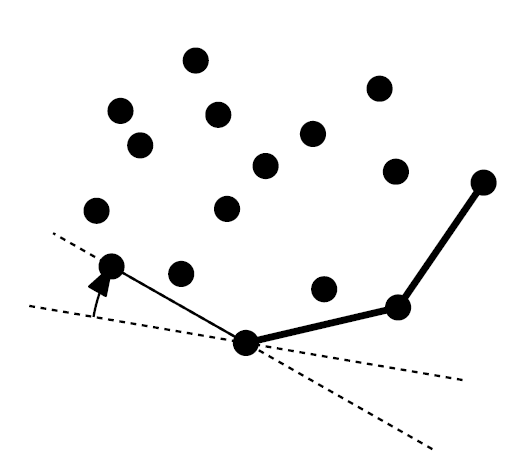
\includegraphics[width=0.3\textwidth]{exercise1}

\begin{enumerate}[a.]
    \item Give pseudocode for this algorithm.
    \item What degenerate cases can occur and how can we deal with them?
    \item Prove that the algorithm correctly computes the convex hull.
    \item Prove that the algorithm can be implemented to run in time $\mathcal{O}(n \cdot h)$, where $h$ is the complexity of the convex hull.
    \item What problems might occur when we deal with inexact floating point arithmetic?
\end{enumerate}

\end{Quest}


\begin{enumerate}[a.]
    \item Algorithm \ref{algo1} 

\begin{algorithm}[ht!] 
    \caption{\textsc{Gift Wrapping Algorithm}}
    \label{algo1}
    \begin{algorithmic}[1]

    \Require A set $P$ of points in the plane.
    \Ensure A list $\mathcal{L}$ containing the vertices of of $\mathcal{CH}(P)$ in clockwise order.
    \Function{jarvis}{$P$}
    
    \State \textit{previous} $\gets$ rightmost point in $P$
    \State $ i \gets 0$
    \Repeat 
            \State $i \gets i+1$
            \State $\mathcal{L}[i] \gets$ \textit{previous}
            \State \textit{next} $\gets P[1]$
            \For{$j$ from $1$ to $|P|$}
                \If {(\textit{next}==\textit{previous}) or ($P[j]$ is on left of line from $\mathcal{L}[i]$ to \textit{next})}
                \State \textit{next} $\gets P[j]$
                \EndIf
            \EndFor
            \State \textit{previous} $\gets$ \textit{next}
        \Until{\textit{next} $== \mathcal{L}[1]$}
    \State \textbf{return} $\mathcal{L}$
    \EndFunction
    \end{algorithmic}
\end{algorithm}

    \item Degeneracies: 
    \begin{itemize}
        \item There could be more than one rightmost point: we use a lexicographic order.
        \item Three of more colinear points: we can choose the point that is farthest among those that are leftmost.
        
        
    \end{itemize}
    \item Proof \cite{l14}: 
    
    Jarvis's March is a straightforward algorithm that computes convex hull for a set of points.  It relies on the following two facts:
    \begin{itemize}
        \item The leftmost point must be one vertex of the convex hull.
        \item If point $p$ is a vertex of the convex hull, then the points furthest clockwise and counter-clockwise are also vertices of the convex hull.
    \end{itemize}
    
    Jarvis's March consists of two stages.
    
    During the first stage (line 2), it finds the rightmost point by comparing the $x$-coordinate.  After it finds the rightmost point, $\mathcal{L}[1]$, \emph{previous} is initialized to that point.
    
    During the second stage, it finds the point that is furthest CCW (counter-clockwise) to \emph{previous}. To do this, it first chooses an arbitrary point $P[1]$, then it iterates over all points to to find the furthest CCW point.  This is very similar to finding the maximum element in an array but here the comparison is not based on numerical values, but on CCW property.

    This process ends when $\mathcal{L}[1]$ becomes the rightmost point again,  at which time the string wraps completely around the set of points. Therefore, this procedure satisfies both facts stated at the beginning of this section. So it correctly finds the convex hull for a set of points

    
    \item Complexity: 
    
    Searching for the rightmost point costs $\mathcal{O}(n)$. After that, for each point belonging to the future convex hull ($h$), we have to evaluate all the other points to find the next hull vertix ($n$). That second part costs $\mathcal{O}(h\cdot n)$. The complexity depends then on the size of the output $h$ and is given by $\mathcal{O}(h\cdot n)$ since $\mathcal{O}(h\cdot n)\geq \mathcal{O}(n)$. 
    
    The worst case is when all points are on the convex hull. In such a case $h=n$ and the complexity becomes $\mathcal{O}(n^2)$.
    
    \item Rounding errors with floating point arithmetic:
    \begin{itemize}
        \item A problem could occur when evaluating if a point is on the left to a segment or not (not robust predicate): a point could be removed from the convex hull although it should be there but structural integrity is unharmed.
    \end{itemize}
\end{enumerate}

\FloatBarrier
\newpage
















%% Exercise 2

\section{}

\begin{Quest}

[2.1] Let $S$ be a set of $n$ disjoint line segments whose upper endpoints lie on the line $y=1$ and whose lower endpoints lie on the line $y=0$. These segments partition the horizontal strip $[- \infty : \infty]\times[0 : 1]$ into $n+1$ regions. Give an $\mathcal{O}(n \log n)$ time algorithm to build a binary search tree on the segments in $S$ such that the region containing a query point can be determined in $O(\log n)$ time. Also describe the query algorithm in detail.

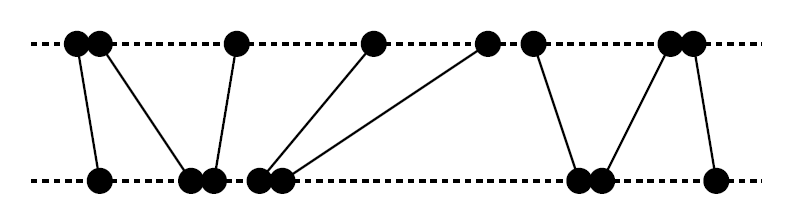
\includegraphics[width=0.5\textwidth]{exercise2}

\end{Quest}

\begin{enumerate}
    \item Build Algorithm \ref{algo2}.
    
    \begin{algorithm}[ht!]
    \caption{\textsc{Build Binary Search Tree Algorithm}}
    \label{algo2}
    \begin{algorithmic}[1]

    \Require A set $S$ of $n$ disjoint line segments whose upper endpoints lie on the line $y=1$ and whose lower endpoints lie on the line $y=0$.
    \Ensure A binary search tree $\mathcal{T}$ on the segments in $S$.
    \Function{Build}{$S$}
    
    \State{$L\gets $ array of the line segments sorted according to the $x$-coordinate of their upper-point.}
    
    \State $ \mathcal{T}\gets $ \textsc{SortedArrayToBST}($L$,$1$,length($L$)) \Comment{Building the tree.}
    
    \State{$i\gets 0$}
    
    \Function{Number}{$T$} \Comment{Giving each leaf a number from left to right.}             
        \If{ $T==leaf$("$0$")}
            \State $i$ $\gets$ $i+1$
            \State \textbf{return} $leaf$("$i$")
        \Else 
            \State $T.left$ $\gets$ \textsc{Number}($T.left$)
            \State $T.right$ $\gets$ \textsc{Number}($T.right$)
            \State \textbf{return} $T$
        \EndIf
    \EndFunction
    
    \State \textbf{return} \textsc{Number}($\mathcal{T}$)
    
    \EndFunction
    
    \Function{SortedArrayToBST}{$L$,$start$,$end$}
    
    \If{($start > end$) }
        \State \textbf{return} $leaf$("$0$")
    \EndIf
    \State{$mid \gets \left\lceil\frac{start+end}{2}\right\rceil$}
    \State{$\mathcal{T} \gets $ new binary tree with key}
    \State{$\mathcal{T}.key \gets L[mid]$}
    \State{$\mathcal{T}.left \gets $ \textsc{SortedArrayToBST}($L$,$start$,$mid-1$)}
    \State{$T.right \gets $ \textsc{SortedArrayToBST}($L$,$mid+1$,$end$)}
    
    \State \textbf{return} $\mathcal{T}$
    \EndFunction
    
    \end{algorithmic}
    \end{algorithm}
    
    \item Complexity: 
    \begin{itemize}
        \item sorting in array $L$ costs $\mathcal{O}(n \log n)$
        \item building the tree is linear in the size of the sorted array: $\mathcal{O}(n)$
        \item  giving each leaf a number costs $\Theta(n)$. 
    \end{itemize}
    Consequently, the time complexity is given by $\mathcal{O}(n \log n)$. 
    \item Query Algorithm \ref{algo2bis}
    
    \begin{algorithm}[ht!]
    \caption{\textsc{Query Algorithm}}
    \label{algo2bis}
    \begin{algorithmic}[1]

    \Require A query point $p$ contained in $[- \infty : \infty]\times[0 : 1]$ and the binary search tree $\mathcal{T}$.
    \Ensure The region $i$ containing the $p$.
    
    \Function{Query}{$p,\mathcal{T}$}
 
        \If{ $\mathcal{T}==leaf$("$x$")} \State \textbf{return} $x$
        \Else
            \If {$p$ is on the left of $\mathcal{T}.key$}
                \State \textbf{return}     \textsc{Query}($p$,$\mathcal{T}.left$)
            \Else
                \State \textbf{return} \textsc{Query}($p$,$\mathcal{T}.right$)
            \EndIf
        \EndIf

    \EndFunction
    
    \end{algorithmic}
    \end{algorithm}

\item Complexity: to get to the final leaf of the three containing the number of the zone containing the query point $p$, we need to go from the root of the balanced tree to its bottom. Since it has at most $\log n$ levels, we have the time complexity $\mathcal{O} (\log n)$. 
    
\end{enumerate}


\FloatBarrier
\newpage














%% Exercise 3

\section{}

\begin{Quest}

[2.14] Let $S$ be a set of $n$ disjoint line segments in the plane, and let $p$ be a point not on any of the line segments of $S$. We wish to determine all line segments of $S$ that $p$ can see, that is, all line segments of $S$ that contain some point $q$ so that the open segment $\overline{pq}$ doesn’t intersect any
$p$ line segment of $S$. Give an $O(n\log n)$ time algorithm for this problem that uses a rotating half-line with its endpoint at $p$.

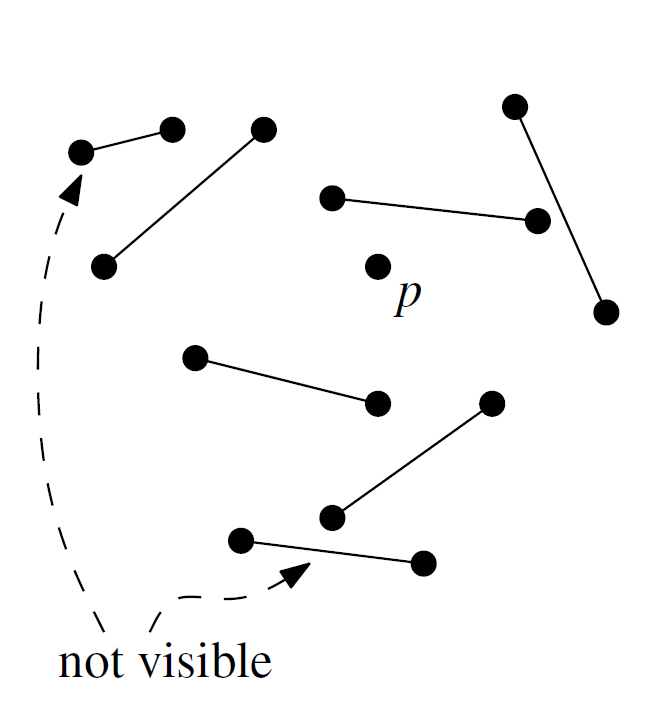
\includegraphics[width=0.3\textwidth]{exercise3}

\end{Quest}
    
\begin{enumerate}[1.]
    \item Algorithm \ref{algo3} \cite{trakla}

    \begin{algorithm}[ht!]
    \caption{\textsc{Rotational Plane Sweep Algorithm}}
    \label{algo3}
    \begin{algorithmic}[1]

    \Require A set $S$ of $n$ disjoint line segments in the plane and a point $p$ not on any of the line segments. 
    \Ensure A subset $\mathcal{S}$ of disjoint line segments that are within line of sight of $p$.
    
        \State $T$, $L$ $\gets$ empty balanced search trees
        \State Sort the vertices  $v_i$ in a set $\mathcal{E}$, according to their clockwise angle $\alpha_i$ that the half-line from $p$ to each vertex $v_i$ makes with the positive x-axis.  In case of ties, sort by increasing distance to $p$.
        \State Let $r$ be the half-line parallel to the positive x-axis starting at $p$. Find the obstacle line segments  that are properly intersected by $r$, and store them in $T$ in the order in which they are intersected by $r$.
        \ForAll{$v$ in $\mathcal{E}$} \Comment {Rotate the half-line to the next vertex.}
            \State {Delete from $T$ the (possible) line segment incident to $v$ that are left to line from $p$ to $v$.}

            \State {Insert into $T$ the (possible) obstacle edge incident to $v$ that are right to line from $p$ to $v$.}
            
            \State $e$ $\gets$ nearest edge of $T$  to $p$.
            
            \If{$e$ is not in $L$}
                \State{Store $e$ in $L$ in the order of the smallest angle made by its endpoints.}
            \EndIf
            
        \EndFor
        
        \State \textbf{return} The set $\mathcal{S}$ containing the line segments of $L$.
 
    
    \end{algorithmic}
    \end{algorithm}
    
    \item Complexity \cite{ex3}
    
    \begin{itemize}
        \item Data structures are linear in number of line segments $n$.
        \item Initial angular sorting: $\mathcal{O}(n \log n)$
        \item Searching $T$ for intersections: $\mathcal{O}(n \log n)$
        \item Number of updates: $\mathcal{O}(n)$
            \begin{itemize}
                \item Updating  $T$: $\mathcal{O}(\log n)$
                \item Storing $e$: $\mathcal{O}(\log n)$
            \end{itemize}
        \item Building the subset $\mathcal{S}$ : $\mathcal{O}(k)$ where $k$ is the size of $L$.
    \end{itemize}
\end{enumerate}

\FloatBarrier
\newpage

















%% Exercise 4


\section{}

\begin{Quest}

[4.2] Consider the casting problem in the plane: we are given polygon $P$ and a 2-dimensional mold for it. Describe a linear time algorithm that decides whether $P$ can be removed from the mold by a single translation.

\end{Quest}


\begin{enumerate}
    \item Algorithm \ref{algo4} \cite{l5}: Every polygon edge requires the removal direction to be in a semi-circle (Figure \ref{fig:cast}). The goal here is thus to compute the common intersection of a set of circular intervals (semi-circles) and check whether it is empty. In fact, we only need to represent upward directions:  we can use points on the line $y=1$.  Indeed, an outward normal $(n_1,n_2)$ to an edge $e$ must form an angle of at least  \SI{90}{degree} with the translation direction $(d,1)$. (Lemma 4.1 p. 65)
    
    $$ n_1 d+n_2\leq 0 \Leftrightarrow \begin{cases}d\geq -\frac{n_2}{n_1} & \text{if } n_1<0 \\ d \in \mathbb{R} & \text{if } n_1=0 \\d\leq -\frac{n_2}{n_1} & \text{if } n_1>0 \end{cases}$$
    
    which means that $d$ must be contained in this half-line. We must thus compute the common intersection of a set of half-lines in 1D. This can be done in three steps:
    \begin{itemize}
        \item Determine the endpoint $p_l$ of the rightmost left-bounded half-line.
        \item Determine the endpoint $p_r$ of the leftmost right-bounded half-line.
        \item The common intersection is [$p_l$, $p_r$] and can be empty.
    \end{itemize}
    
    
\begin{figure}[ht] 
  \label{fig:cast} 
  \begin{minipage}[b]{0.5\linewidth}
    \centering
    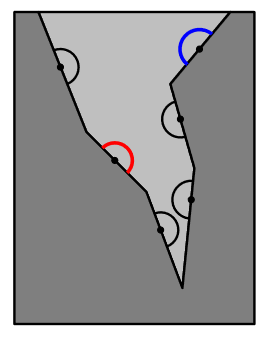
\includegraphics[width=.7\linewidth]{castingpolyhedron1}
    \caption{2D representation of the directions.} 
    \vspace{4ex}
  \end{minipage}%%
  \begin{minipage}[b]{0.5\linewidth}
    \centering
    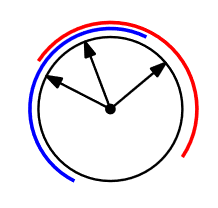
\includegraphics[width=.7\linewidth]{castingpolyhedron2}
    \caption{Common intersection of a set of circular intervals.} 
    \vspace{4ex}
  \end{minipage} 
  \begin{minipage}[b]{0.5\linewidth}
    \centering
    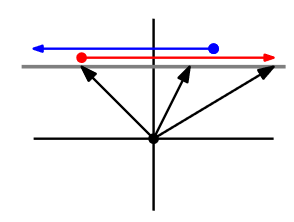
\includegraphics[width=.7\linewidth]{castingpolyhedron3}
    \caption{We can use points on the line $y=1$.} 
    \vspace{4ex}
  \end{minipage}%% 
  \begin{minipage}[b]{0.5\linewidth}
    \centering
    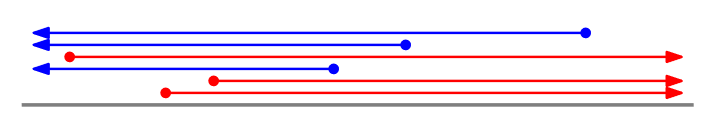
\includegraphics[width=.7\linewidth]{castingpolyhedron4}
    \caption{The common intersection of a set of half-lines in 1D.} 
    \vspace{4ex}
  \end{minipage} 
\end{figure}

    \begin{algorithm}[ht!]
    \caption{\textsc{Casting a Polyhedron}}
    \label{algo4}
    \begin{algorithmic}[1]

    \Require A set $S$ of the $n$ segments constituting the mold + top facet.
    \Ensure $true$ if the polygon can be removed with a single translation and $false$ otherwise.
    \State $L \gets$ empty list, $k_l \gets 0$
    \State $R \gets$ empty list, $k_r \gets 0$
    \For {$i = 1:n$} \Comment{Compute the half-lines}
        \State {$(n_1,n_2)$ $\gets$ the outward normal to $S(i)$}
        \If{$n_1<0$}
            \State $k_l \gets k_l+1$
            \State{$L(k_l) \gets -\frac{n_2}{n_1}$}
        \EndIf
        \If{$n_1>0$}
            \State $k_r \gets k_r+1$
            \State{$R(k_r) \gets -\frac{n_2}{n_1}$}
        \EndIf
    \EndFor
    \State $l$ $\gets$ $-\infty$
    \State $r$ $\gets$ $+\infty$
    \For {$i = 1:k_l$} \Comment{Compute the rightmost left bound.}
            \If{$l<L(i)$}
                \State{$l \gets L(i)$}
            \EndIf
    \EndFor
    \For {$i = 1:k_r$} \Comment{Compute the leftmost right bound.}
            \If{$r>R(i)$}
                \State{$r \gets R(i)$}
            \EndIf
    \EndFor
      \State \textbf{return} $l<=r$
    \end{algorithmic}
    \end{algorithm}
    

    \item Complexity:  The algorithm takes only $\mathcal{O}(n)$ time for $n$ half-lines. No sorting is needed.
    
\end{enumerate}


\FloatBarrier
\newpage

















%% Exercise 5

\section{}

\begin{Quest}

[5.1] In the proof of the query time of the kd-tree we found the following recurrence:
$$ Q(n) = \begin{cases} \mathcal{O}(1), & \text{ if } n = 1,\\
2+2 Q(n/4), & \text{ if } n > 1.
\end{cases}$$
\begin{enumerate}
    \item Prove that this recurrence solves to $Q(n) = \mathcal{O}(\sqrt{n})$. 
    \item Also show that $\Omega(\sqrt{n})$ is a lower bound for querying in a kd-tree by defining a set of $n$ points and a query rectangle appropriately.
\end{enumerate}

\end{Quest}

\begin{enumerate}
    \item Assuming $n=2^{2k}$:
    \begin{align*}
        Q(n)&=2 + 2 Q(n/4)\\
        &=2 + 2 Q(2^{2(k-1)})\\
        &=2 + 2 \left[ 2+ 2Q(2^{2(k-2)}) \right]=2 + 2^2 + 2^2 Q(2^{2(k-2)})\\
        &=2 + 2^2 + 2^3+ 2^3 Q(2^{2(k-3)})\\
        \intertext{Using geometric serie formula and $\sqrt{n}=2^{k}$:}
        &=2 \frac{2^k-1}{1} + 2^k Q(2^{2(k-k)})\\
        &=2 \frac{2^k-1}{1} + 2^k c\\
        &=2^{k+1}-2+ 2^kc\\
        &=2(2^{k}-1)+2^k c\\
        &=2(\sqrt{n}-1)+c \sqrt{n}\\
        &=\mathcal{O}(\sqrt{n})
    \end{align*}
    \item /
\end{enumerate}

\FloatBarrier
\newpage













%% Exercise 6

\section{}

\begin{Quest}

[6.7] A polygon $\mathcal{P}$ is called \textit{star-shaped} if a point $p$ in the interior of $\mathcal{P}$ exists such that, for any other point $q$ in $\mathcal{P}$, the line segment $\overline{pq}$ lies in $\mathcal{P}$. Assume that such a point $p$ is given with the star-shaped polygon $\mathcal{P}$. As in the previous two exercises the vertices of $\mathcal{P}$ are given in sorted order along the boundary in an array. 
\begin{enumerate}
    \item Show that, given a query point $q$, it can be tested in time $\mathcal{O}(\log n)$ whether $q$ lies inside $\mathcal{P}$. 
    \item What if $\mathcal{P}$ is star-shaped, but the point $p$ is not given?
\end{enumerate}

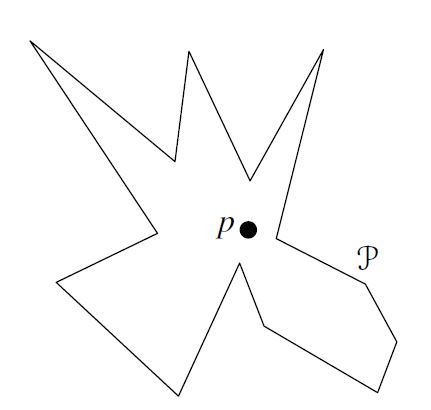
\includegraphics[width=0.3\textwidth]{exercise6}

\end{Quest}


\begin{enumerate}[1.]
    \item Algorithm \ref{algo6} \cite{hw3}: Since every point within the polygon is visible from point $p$, we can divide the polygon into triangles by drawing a segment from $p$ to each of the polygon's vertices. Then a binary search will locate the proper cone in logarithmic time. Some precautions must be taken because the search range is circular, but binary search is designed for linear ranges \cite{circ}. Then a constant-time test will determine on which side of the perimeter edge the query point lies.
    
     \begin{algorithm}[ht!]
    \caption{\textsc{Query Point In Kernel Of Star Shaped Polygon}($S$,$q$,$p$)}
    \label{algo6}
    \begin{algorithmic}[1]

    \Require A list $S$ of the $n$ vertices of a star-shaped polygon $\mathcal{P}$ in counter-clockwise order along the boundary, a point $p$ in the interior of $\mathcal{P}$ and a query point $q$ in the plane $\mathbb{R}^2$.
    \Ensure $true$ if the polygon $\mathcal{P}$ contains $q$ and $false$ otherwise.
    
    \State{$e_2 \gets$ \textsc{MinAngleSearch}( $S$,$1$,$n$,$q$,$p$)} \Comment{Search for the half-line $[pS[e_2]$ that makes the smallest angle with $[pq$ in the counterclockwise order.}
    \If{ $e_2==1$}
        \State $e_1 \gets n$
    \Else
        \State $e_1 \gets e_2-1$
    \EndIf
    \If{ $q$ is on the right side of $S[e_1]S[e_2]$} 
        \State \textbf{return} $false$
    \Else
        \State \textbf{return} $true$
    \EndIf \Comment{Check if the point is within the triangle.}
    
    \Function{MinAngleSearch}{$A$,$low$,$high$,$q$,$p$}
        \If{$high==low$} 
            \State \textbf{return} $low$
        \EndIf \Comment{If there is only one element left.}
        \State{$mid \gets \left\lceil \frac{low+high}{2} \right\rceil$} \Comment{Find mid.}
        \If{$mid < high \text{ and }  \angle(pq,pA[mid+1])< \angle(pq,pA[mid])$} 
            \State {\textbf{return} $mid+1$}
        \EndIf \Comment{Check if element ($mid+1$) is minimum element.}
        \If{$mid > low \text{ and } \angle(pq,pA[mid])< \angle(pq,pA[mid-1])$} 
            \State { \textbf{return} $mid$ }
        \EndIf \Comment{Check if $mid$ itself is minimum element.}
        \If{$\angle(pq,pA[mid])< \angle(pq,pA[high])$} 
            \State{\textbf{return} \textsc{MinAngleSearch}($A$,$low$,$mid-1$,$q$,$p$)}
        \Else
            \State{\textbf{return} \textsc{MinAngleSearch}($A$,$mid+1$,$high$,$q$,$p$)}
        \EndIf \Comment{Decide whether we need to go to left half or right half.}
    \EndFunction
    \end{algorithmic}
    \end{algorithm}
    
    \item When $p$ is not given \cite{hw3}: 
    
    We know that the algorithm computing a trapezoidal map $\mathcal{T}(S)$ of a set $S$  of $n$ line segments and the corresponding search structure $\mathcal{D}$ has an expected time of $\mathcal{O}(n\log n)$ and the search algorithm an expected time of $\mathcal{O}(\log n)$. Therefore, it would more interesting to find an interior point $p$ in $\mathcal{O}(n)$ and to apply the previous search in $\mathcal{O}(\log n)$. Since we have the $n$ vertices of a star-shaped polygon $\mathcal{P}$ in sorted order along the boundary, it is possible.

    An easy solution is the following: to each edge of the perimeter corresponds a partition into half planes and by turning around the perimeter, a consistent orientation for these partitions is determined. If a special point $p$ exists, then it must be on the same side of every one of these partitions, so it suffices to intersect all "inside" half-planes determined by the edges of the polygon. If the result is empty, then the claim that the polygon was star-shaped was false; otherwise, any point within the convex polygon that is the intersection is a valid choice. 

    It can be found in linear time. The algorithm is not even that complex: go around the perimeter and compute on the fly the intersection of the half-planes defined by the edges seen so far, but a simple incremental computation. The trick is that intersecting the existing intersection polygon with the next half-plane can be done in amortized constant time, because we know a lot about the next half-plane. We shall maintain the tangency points to the current intersection from the next vertex on the perimeter of the given polygon and use them in handling the next edge; note that maintaining these tangency points is simply a matter of turning around the (convex) intersection figure and, in the worst case, will have required us to turn all the way around the intersection figure through the execution of the algorithm, which clearly takes linear time overall and thus constant amortized time per operation. With the help of the tangency points, it is a simple matter to compute the intersection with the new half-plane, again by walking the boundary of the current intersection polygon, and again for a total cost of $\mathcal{O}(n)$ overall. 
    
\end{enumerate}

\FloatBarrier
\newpage











\bibliographystyle{unsrt}
\bibliography{mybib.bib}

\end{document}
